\documentclass[12pt,a4paper]{scrartcl}

%========================================================================================
%SPRACHE

\usepackage[ngerman]{babel} 
\usepackage[T1]{fontenc} 				% richtige Silbentrennung
\usepackage[utf8]{inputenc}    % Umlaute etc.!!! BENUTZEN!!!!
\usepackage{float} % alles möglichen Sachen mit [h] an die richtige Stelle zwingen
%\usepackage{rotating} % tabellen rotieren
%\usepackage{supertabular} % schraege tabellen etc
%\usepackage{pdfpages}     % pdfs einbinden


\usepackage[]{natbib}

%========================================================================================
%DARSTELLUNG

\usepackage[small,compact]{titlesec} 		% Verkleinerung von Section-Ueberschriften
\usepackage{graphicx}				  	% Einbinden von Graphiken .ps, .pdf, .png

\usepackage{amsmath}					% mathematische Symbole
%\usepackage {ulem} 						%\emph{Text}: Text wird unterstrichen
\setlength{\parindent}{0pt}				% Zeile nach Absatz einruecken 1pt oder nicht 0pt.

%========================================================================================
%FARBEN

%\usepackage[usenames,dvipsnames]{color}	

									%Apricot 	Aquamarine 	Bittersweet 	Black
									%Blue 	BlueGreen 	BlueViolet 	BrickRed
									%Brown 	BurntOrange 	CadetBlue 	CarnationPink
									%Cerulean 	CornflowerBlue 	Cyan 	Dandelion
									%DarkOrchid 	Emerald 	ForestGreen 	Fuchsia
									%Goldenrod 	Gray 	Green 	GreenYellow
									%JungleGreen 	Lavender 	LimeGreen 	Magenta
									%Mahogany 	Maroon 	Melon 	MidnightBlue
									%Mulberry 	NavyBlue 	OliveGreen 	Orange
									%OrangeRed 	Orchid 	Peach 	Periwinkle
									%PineGreen 	Plum 	ProcessBlue 	Purple
									%RawSienna 	Red 	RedOrange 	RedViolet
									%Rhodamine 	RoyalBlue 	RoyalPurple 	RubineRed
									%Salmon 	SeaGreen 	Sepia 	SkyBlue
									%SpringGreen 	Tan 	TealBlue 	Thistle
									%Turquoise 	Violet 	VioletRed 	White
									%WildStrawberry 	Yellow 	YellowGreen 	YellowOrange
									
									% verwenden mit: 
									% \pagecolor{declared-color}
									% {\color{declared-color} text}
									% \colorbox{declared-color1}{\color{declared-color2} text}
									%========================================================================================
%Zur Einbindung von Programmiertexten mit:
				% \begin{lstlisting}
				%put your code here
				%\end{lstlisting}
				
\usepackage{listings}
\lstset{ %
language=Matlab,                			% the language of the code
basicstyle=\footnotesize,       			% the size of the fonts that are used for the code
numbers=left,                   				% where to put the line-numbers
numberstyle=\footnotesize,      			% the size of the fonts that are used for the line-numbers
stepnumber=2,                   				% the step between two line-numbers. If it's 1, each line 
                                					% will be numbered
numbersep=5pt,                  			% how far the line-numbers are from the code
backgroundcolor=\color{white},  		% choose the background color. You must add \usepackage{color}
showspaces=false,               			% show spaces adding particular underscores
showstringspaces=false,        		 	% underline spaces within strings
showtabs=false,                 				% show tabs within strings adding particular underscores
frame=single,                   				% adds a frame around the code
tabsize=2,                      				% sets default tabsize to 2 spaces
captionpos=b,                   				% sets the caption-position to bottom
breaklines=true,                				% sets automatic line breaking
breakatwhitespace=false,        			% sets if automatic breaks should only happen at whitespace
title=\lstname,                 				% show the filename of files included with \lstinputlisting;
                                					% also try caption instead of title
}
%========================================================================================


%LOAD FANCYHDR fuer Kopf- und Fu{\ss}zeilen
%\usepackage{fancyhdr}					% Paket laden	f\"ur einfache Handhabung von Kopf-und Fu{\ss}zeile
%\fancyhf{}								% alle Kopf- und Fu{\ss}zeilen bereinigen
%\pagestyle{fancy}						% Deklariere Seitenstil
%----------------------------------------------------------------------------------------------------------------------------------------------------------
% Angaben fuer Kopf-und Fu{\ss}zeilen links[L] und rechts[R]		
%\fancyhead[L]{{\textbf{Entwicklung eines Schwingungsmesssystems für ein Radar}}}
%\fancyfoot[C]{\thepage} 					% Seitennummer unten mittig

\usepackage[headsepline,plainheadsepline]{scrpage2}
\pagestyle{scrheadings}
\ihead[\rightmark]{\rightmark} \chead[]{}
\ohead[\pagemark]{\pagemark} \cfoot[]{}

\automark{section}
\renewcommand{\sectionmark}[1]{\markright{\ #1}}


\usepackage[small, nooneline, bf]{caption}

\addto\captionsngerman{
\renewcommand{\figurename}{Abb.}
\renewcommand{\tablename}{Tab.}
}

\usepackage{booktabs}



%==========================================================================================

\begin{document}
\title {Entwicklung eines Schwingungsmesssystems für ein Radar}
\author{Sebastian Beyer}
\maketitle

\newpage

\tableofcontents
\newpage


\section{Abstrakt}

\newpage

\section{Motivation und Hintergrund}

\newpage

\section{Hintergrund: Beschleunigungssensoren}

Beschleunigungssensoren messen grundsätzlich die Kraft, die auf ein System wirkt. Diese setzt sich aus der Gravitation und Trägheitskräften zusammen. Isoliert man die Trägheitskräfte, so lässt sich daraus die Translationsbeschleunigung bestimmen. Mithilfe dieser lässt sich die Positionsänderung des Systems berechnen. (Referenz?)\\

Es gibt verschiedene Prinzipien, mit denen die Beschleunigung bestimmt werden kann. Das verbreitetste ist das der Federwaage.

\begin{figure}[H]
\centering
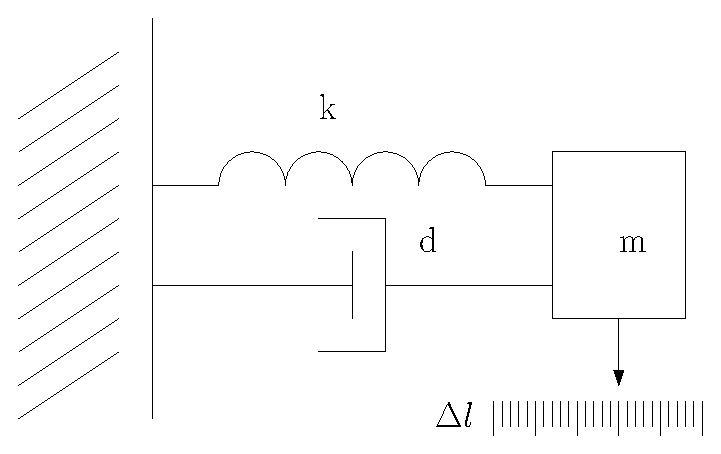
\includegraphics[scale=0.7]{federmasse.eps}
\caption{Masse-Feder-System zur Beschleunigungsmessung. k, d, m und $\Delta l$ bezeichnen Federkonstante, Dämpfung, Masse und Auslenkung. nach \citep{Klingbeil:2006qy}.}
\label{federwaage}
\end{figure}

Eine Masse m (auch seismische Masse genannt) ist über einer Feder mit der Federkonstante k mit einem festen Bezugspunkt verbunden. Die Auslenkung $\Delta l$ ist proportional zur auf die Masse wirkenden Beschleunigung a.
\begin{equation}
a = \frac{k}{m} \cdot \Delta l
\end{equation}

Zu beachten ist die Ausrichtung des Sensors, a entspricht immer der Projektion der Beschleunigung auf die Auslenkungsrichtung von m.\\
Durch geeignete Wahl von k, d und m lässt sich das System für den jeweiligen Fall so einstellen, dass die Ansprechzeit, Resonanz und Sensitivität optimal sind und es möglichst zu keinerlei Nachschwingen kommt. \\

Mittlerweile sind Beschleunigungssensoren in den meisten Fällen als MEMS realisiert (\textbf{M}icro \textbf{E}lectro \textbf{M}echanical \textbf{S}ystems). Sehr kleine mechanische Elemente (1-100 Mikrometer) werden zusammen mit elektronischen Schaltungen auf einen Siliziumwafer aufgebracht. Dabei werden Techniken aus der Fabrikation von integrierten Schaltkreisen (ICs) verwendet, was dazu führt, dass komplizierte elektromechanische System in winziger Größe und hoher Stückzahl hergestellt werden können. Der geringe Preis führt dazu, dass die Sensoren in mehr und mehr Anwendungen integriert werden (Autos, Smartphones, Quadrokopter…).

Die Messung der Auslenkung erfolgt im Wesentlichen durch zwei Verfahren:

\subsection{Piezoresistive Sensoren}
Piezoresistive Sensoren machen sich den Piezoelektrischen Effekt zunutze. In der Feder der Testmasse befinden sich Piezoelemente, welche sich bei Auslenkung verformen und damit ihren Widerstand ändern. Silizium ist ein geeignetes Material, da es sehr empfindlich und linear reagiert und gleichzeitig gut mit der MEMS Technik kombinierbar ist \citep{Kanda:1991gf}.

\subsection{Kapazitative Sensoren}

\begin{figure}[htb]
\begin{minipage}[H]{8cm}
	\centering
	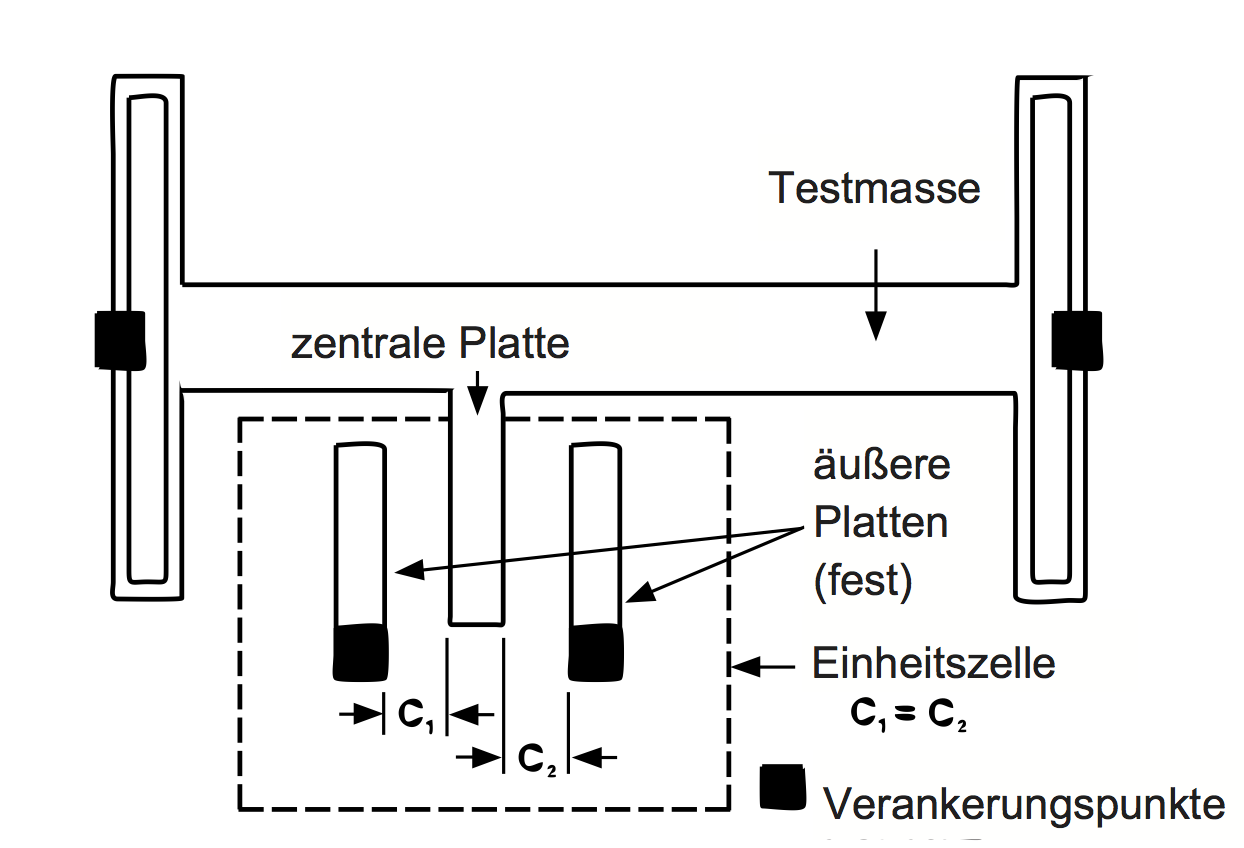
\includegraphics[width=8cm]{adxl_ruhe.png}
	\caption{Vereinfachtes Diagramm des ADXL05 in Ruhe \citep{Devices:1996pd}}
	\label{adxl_ruhe}
\end{minipage}
\hfill
\begin{minipage}[H]{8cm}
	\centering
	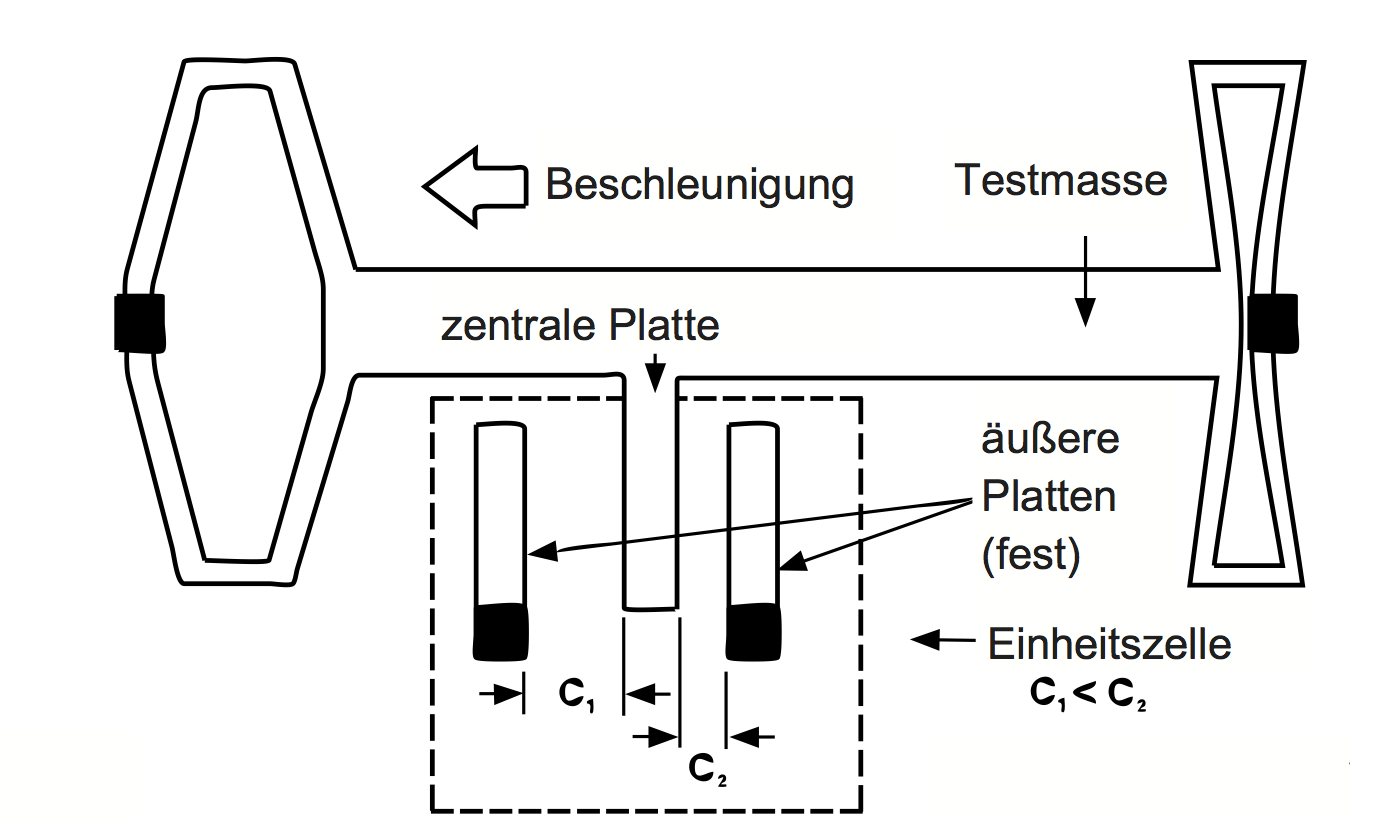
\includegraphics[width=8cm]{adxl_action.png}
	\caption{Vereinfachtes Diagramm des ADXL05 während einer externen Beschleunigung \citep{Devices:1996pd}}
	\label{adxl_action}
\end{minipage}
\end{figure}

\begin{figure}[htb]
\centering
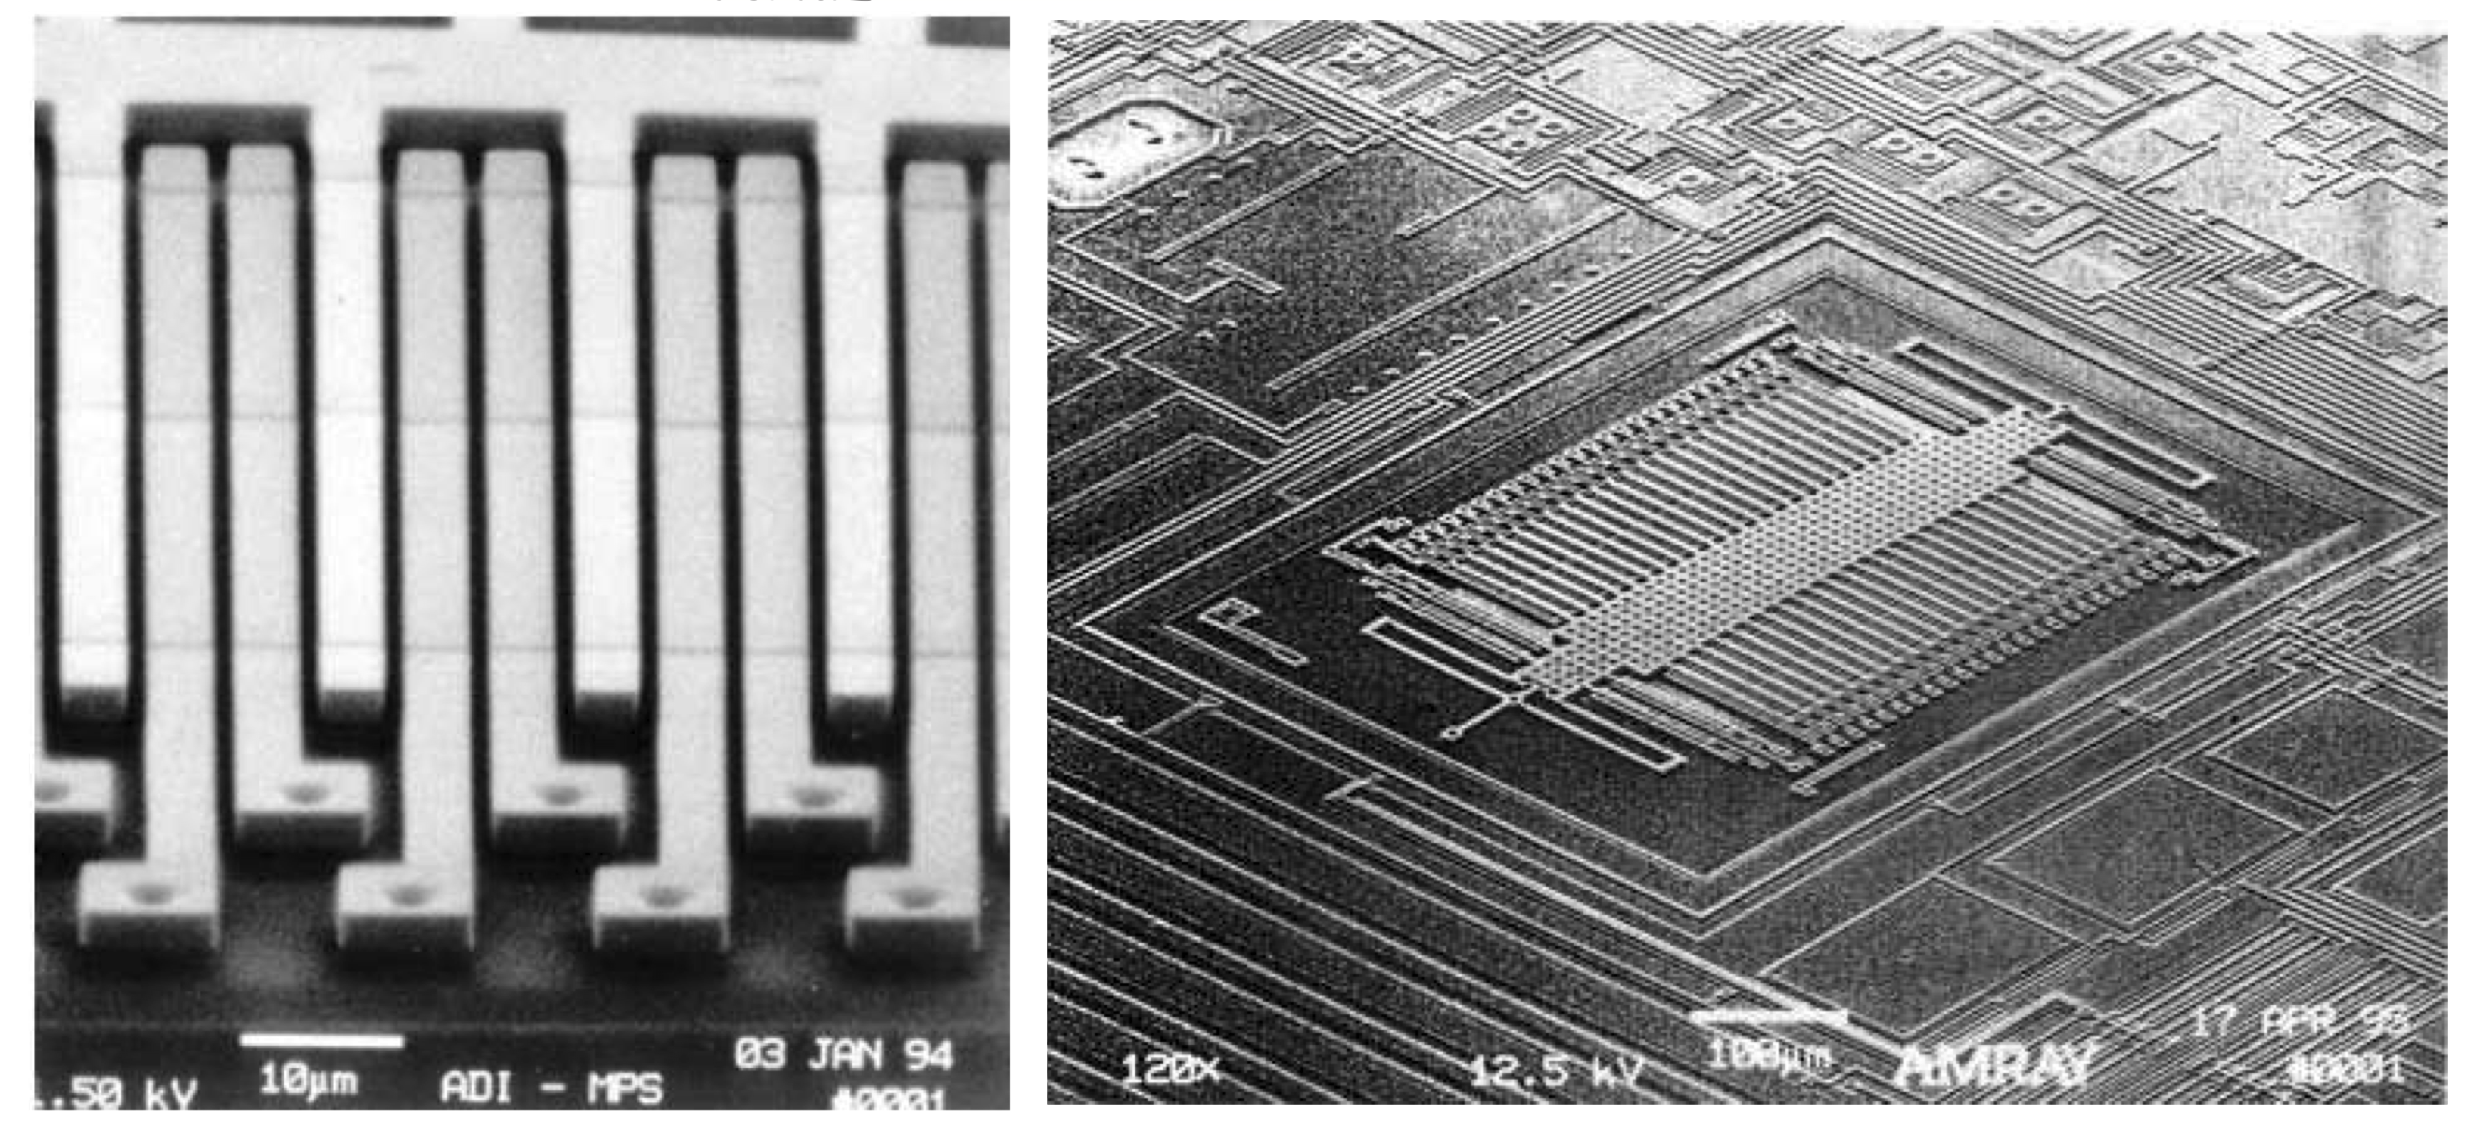
\includegraphics[scale=1]{adxl_micro.png}
\caption{ADXL05 unter dem Elektronenmikroskop, Beispiel für einen kapazitativen MEMS Beschleunigungssensor mit 46 Einzelzellen \citep{Klingbeil:2006qy}.}
\label{adxl_micro}
\end{figure}



Die Auslenkung lässt sich auch über eine Kapazitätsmessung bestimmen, wenn man je eine Elektrode an der Testmasse und eine am fixen Referenzpunkt anbringt.\citep{S.J.-Sherman:1992ul} Eine mögliche Realisierung ist in Abbildung \ref{adxl_ruhe} und Abbildung \ref{adxl_action} zu sehen: Es handelt sich um einen sogenannten Differentialkondensatorsensor. Der Vorteil bei dieser Art von Sensoren ist die Möglichkeit zur Linearisierung und Kompensation \citep{:2002fk}. (ERKLÄREN??) \\
Die seismische Masse befindet sich zwischen zwei fest verankerten Platten, die zusammen zwei Kondensatoren $C_1$ und $C_2$ bilden (Abbildung \ref{adxl_ruhe}). Eine auftretende Beschleunigung führt also zu einer Auslenkung der Mittelelektrode des Kondensatorenpaares (seismische Masse) um die Länge $\pm \Delta l$ und damit zu einer symmetrischen Kapazitätsänderung um $\pm \Delta C$ (Abbildung \ref{adxl_action}).

Um diese Variation in ein elektrisches Ausgangssignal umzusetzen, wird eine sogenannte Brückenschaltung verwendet (Abbildung \ref{bruecke}).

\begin{figure}[H]
\centering
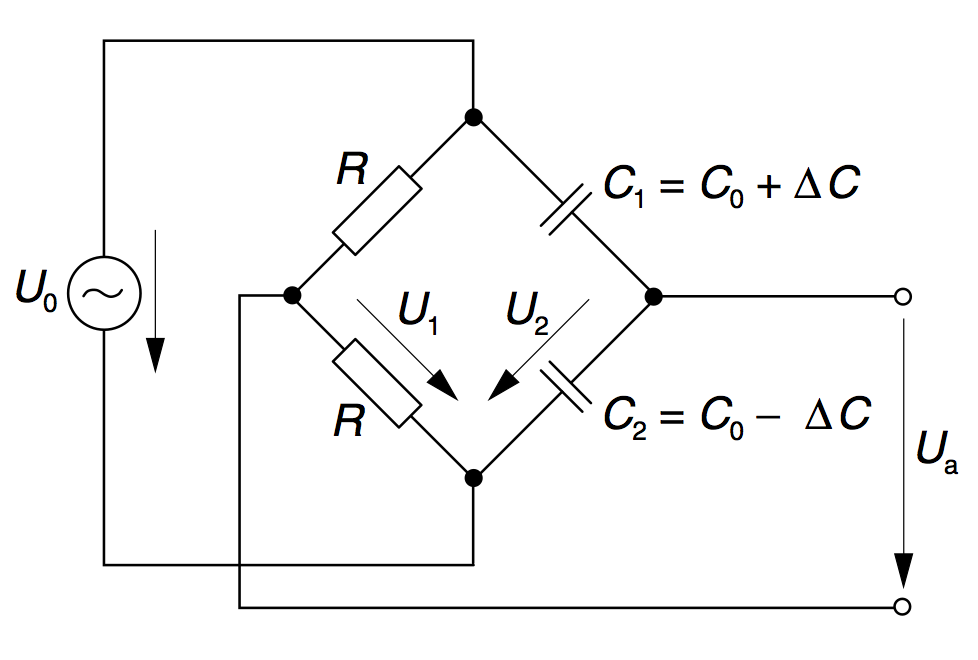
\includegraphics[scale=2]{schaltung_beschleunigungssensor.png}
\caption{Brückenschaltung mit Differentialkondensator (Die mit $U_a$ verbundenen Elektroden von $C_1$ und $C_2$ bilden eine gemeinsame Platte) \citep{:2002fk}}
\label{bruecke}
\end{figure}

Wird nun eine Wechselspannung an die Brücke angelegt, so ergibt sich nach der Spannungsteilerregel für den Ausgang $U_a$:

\begin{equation}
U_a = U_1 - U_2 = U_0 \frac{R}{2 R} - U_0 \dfrac{\dfrac{1}{j \omega C_2} } { \dfrac{1} {j \omega C_2} + \dfrac{1}{j \omega C_1} }
\end{equation}

Durch Kürzen ergibt sich:

\begin{equation}
U_a = \frac{U_0}{2} - U_0 \dfrac{\dfrac{1}{C_2}}{\dfrac{1}{C_2} + \dfrac{1}{C_1}} = U_0 \left( \frac{1}{2} - \frac{C_1}{C_2 + C_1} \right) = \frac{U_0}{2} \left( \frac{C_2 - C_1}{C_2 + C_1} \right)
\end{equation}

Mit $C_1 = C_0 + \Delta C = \varepsilon _0 \cdot \varepsilon _r \cdot A / (d_0 - \Delta l )$ und $C_2 = C_0 - \Delta C = \varepsilon _0 \cdot \varepsilon _r \cdot A / (d_0 + \Delta l )$ erhält man eine lineare Abhängigkeit der Ausgangsspannung $U_a$ von der Auslenkung  $\Delta l$:

\begin{equation}
U_a = - U_0 \frac{\Delta l}{2 d_0}
\end{equation}

Aus \citep{:2002fk}.\\

Diese Spannung lässt sich nun digitalisieren und auslesen. In vielen MEMS Bausteinen ist bereits ein integrierter Analog Digital Wandler eingebaut, sodass die Messwerte direkt digital abrufbar sind. 

\newpage

\section{Entwicklung des ersten Schwingunsmesssystems (BMA180)}

Um abschätzen zu können wie groß die auftretenden Beschleunigungen an der Radarantenne sind, habe ich damit begonnen einen günstigen, schnell zu verwendenden Prototypen zu entwickeln. Dies ist vor Allem wichtig, um entscheiden zu können, für welchen Messbereich und welche Frequenzen der eigentliche Sensor ausgelegt sein muss. \\

\subsection{Bosch BMA180}
\begin{figure}[h]
\centering
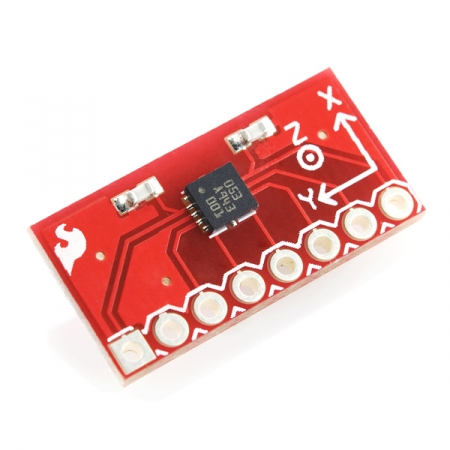
\includegraphics[scale=.4]{hardwareimages/bma180_breakout.jpg}
\caption{BMA180 Breakoutboard von Sparkfun}
\label{bma180_breakout}
\end{figure}

Die Wahl fiel auf einen \textit{Bosch BMA180} digitalen, dreiachsigen MEMS Beschleunigungssensor. Er verfügt über einen eingebauten 14-bit Analog-Digital Wandler und sieben per Software verstellbaren Messbereiche von $\pm1$ bis $\pm16$g.
Die Kommunikation kann über SPI oder I2C erfolgen.

Ich nutze ein Breakoutboard von Sparkfun, da so das knifflige SMD-Löten entfällt und bereits zwei Spannungsstabilisierende Kondensatoren eingebaut sind.

\subsection{Arduino}

\begin{figure}[h]
\centering
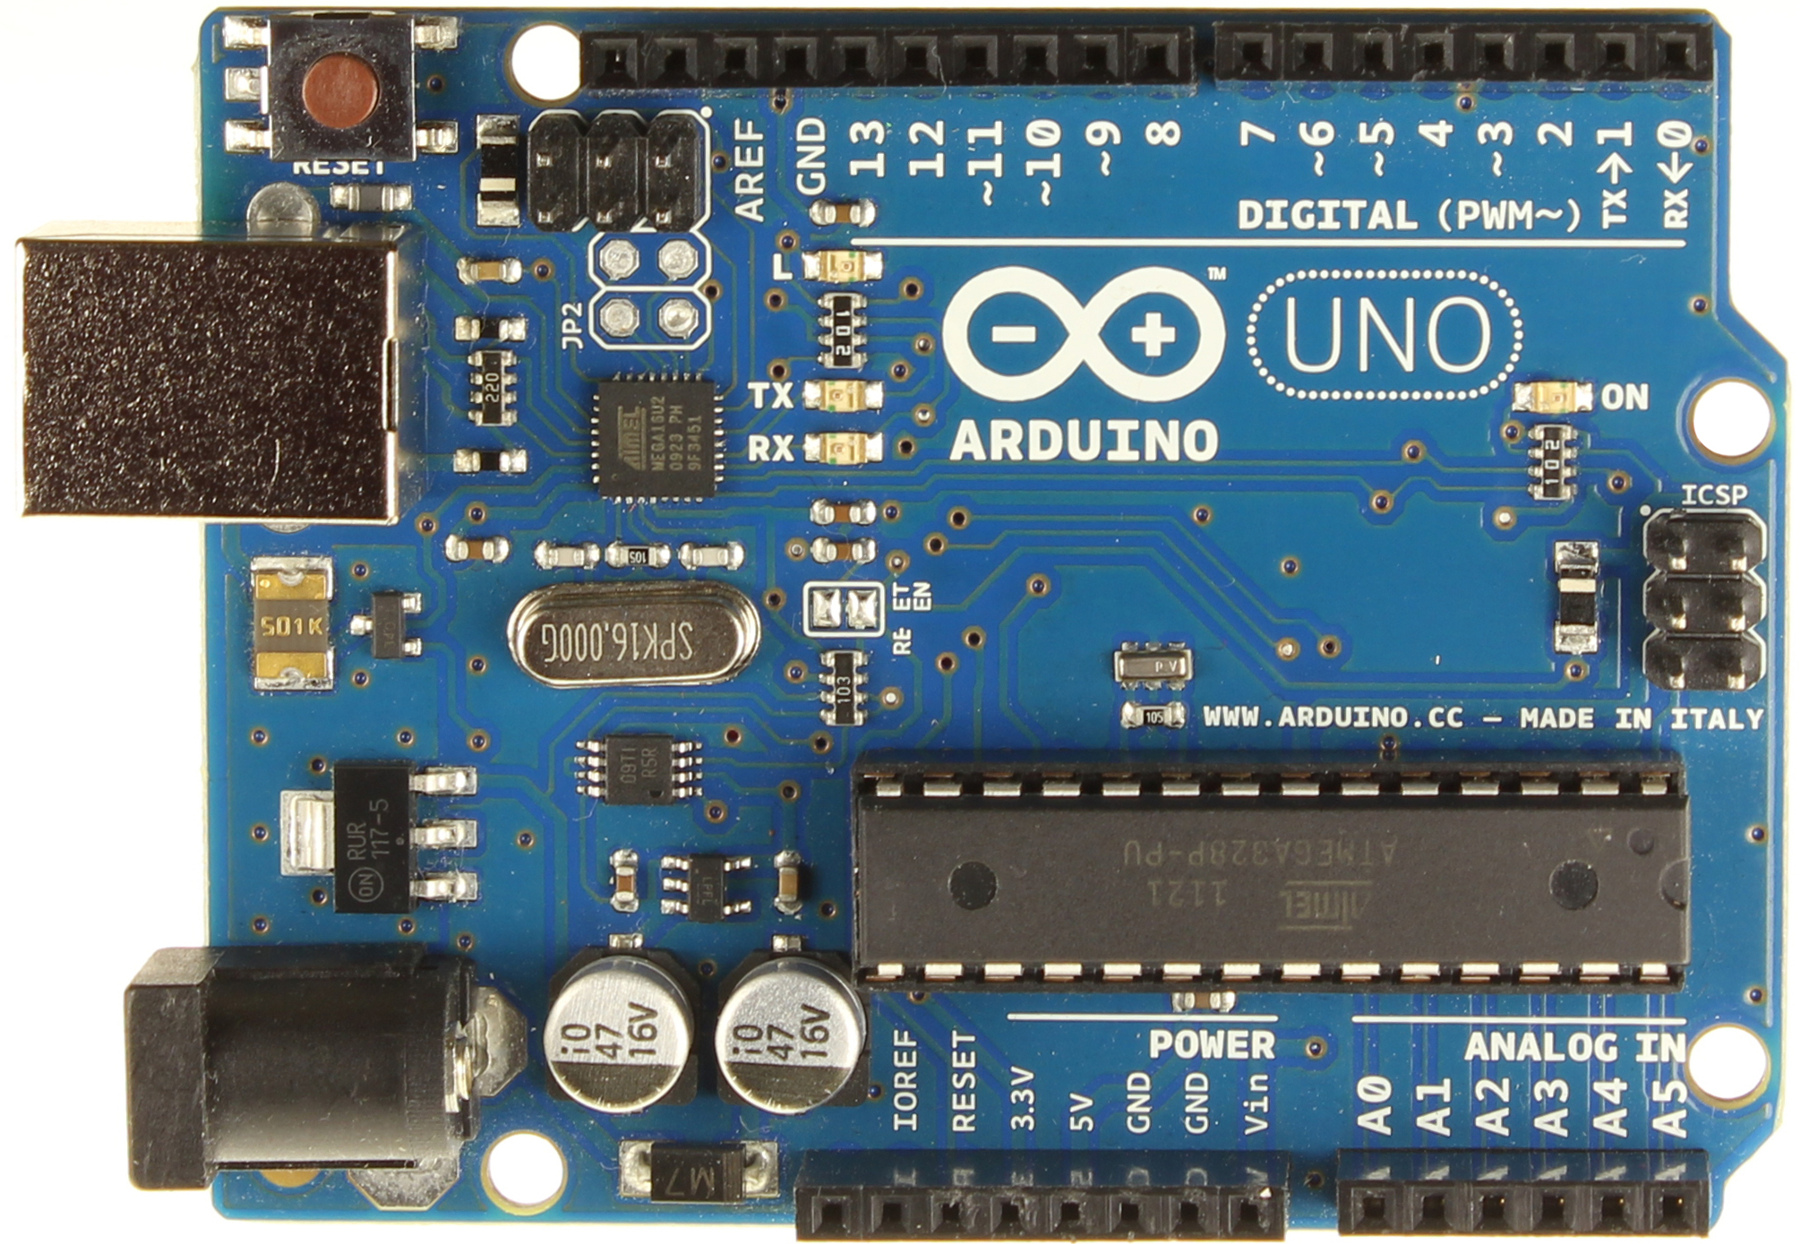
\includegraphics[scale=.2]{hardwareimages/ArduinoUno_R3_Front.jpg}
\caption{Arduino UNO}
\label{Arduino}
\end{figure}


Arduino ist eine auf Atmega Mikroprozessoren basierende Open-Source Entwicklungsplattform zur Verarbeitung von analogen und digitalen Signalen. Die Programmierung kann über eine eigene Entwicklungsumgebung in einer an \textit{Processing\footnote{LINK?}} angelehnten Sprache erfolgen, die im Prinzip ein vereinfachtes C/C++ darstellt.\\
Die Plattform ist auf Prototyping und Experimente ausgelegt. Es ist bereits ein Bootloader vorinstalliert, so kann die Programmierung direkt über die serielle Schnittstelle erfolgen. Die Boards machen die meisten Pins des Atmegas für eigene Schaltungen verfügbar, in den gängigen Boards sind das 14 Pins, die frei als Ein- oder Ausgänge genutzt werden können.
Die Stromversorgung kann über USB oder eine externe 5V Quelle erfolgen. Als weitere Interfaces werden SPI, ICSP und I2C angeboten.

\subsection{Schnittstellen}

\subsubsection{I$^2$C}
Die Kommunikation zwischen Beschleunigungssensor und Arduino erfolgt über den  I$^2$C Bus.
Dabei handelt es sich um einen von Phillips entwickelten seriellen Datenbus, der ursprünglich entwickelt wurde, um Chips in Fernsehgeräten steuern zu können. Inzwischen ist das Patent ausgelaufen und er wird in vielen Hardwareprojekten verwendet, da er sehr leicht zu verstehen und zu verwenden ist. 
\citep{:2012fj}
\subsubsection{Serieller Port}
Zum einfachen Anschluss des Arduinos an einen PC oder Datenlogger wird eine serielle Schnittstelle nach RS232 (REFERENZ) verwendet. Auf dem Arduino befindet sich ein ATmega16U2, welcher die seriellen Signale in USB umwandelt und dafür sorgt, dass der Arduino am PC als virtueller COM-Port erscheint.

\newpage
\subsection{Aufbau und Schaltung}

\subsubsection{Testaufbau}

Um die korrekte Verschaltung zu überprüfen und die Software für das Auslesen der Daten zu zu entwickeln, habe ich zunächst auf dem Breadboard gearbeitet. Der dazu verwendete Schaltplan ist in Abbildung \ref{schematics} zu sehen.

Da der Sensor im I$^2$C Modus betrieben werden soll, ist CS auf High (3.3V) geschaltet. Der SDO-Pin setzt damit dann die Adresse des Chips, wie aus Tabelle \ref{i2cmode} zu entnehmen ist. Ist dieser Low (GND), so ist die Adresse 0x40.



\begin{figure}[h]
\centering

\end{figure}

\begin{figure}[htb]
\begin{minipage}[H]{8cm}
	\centering
	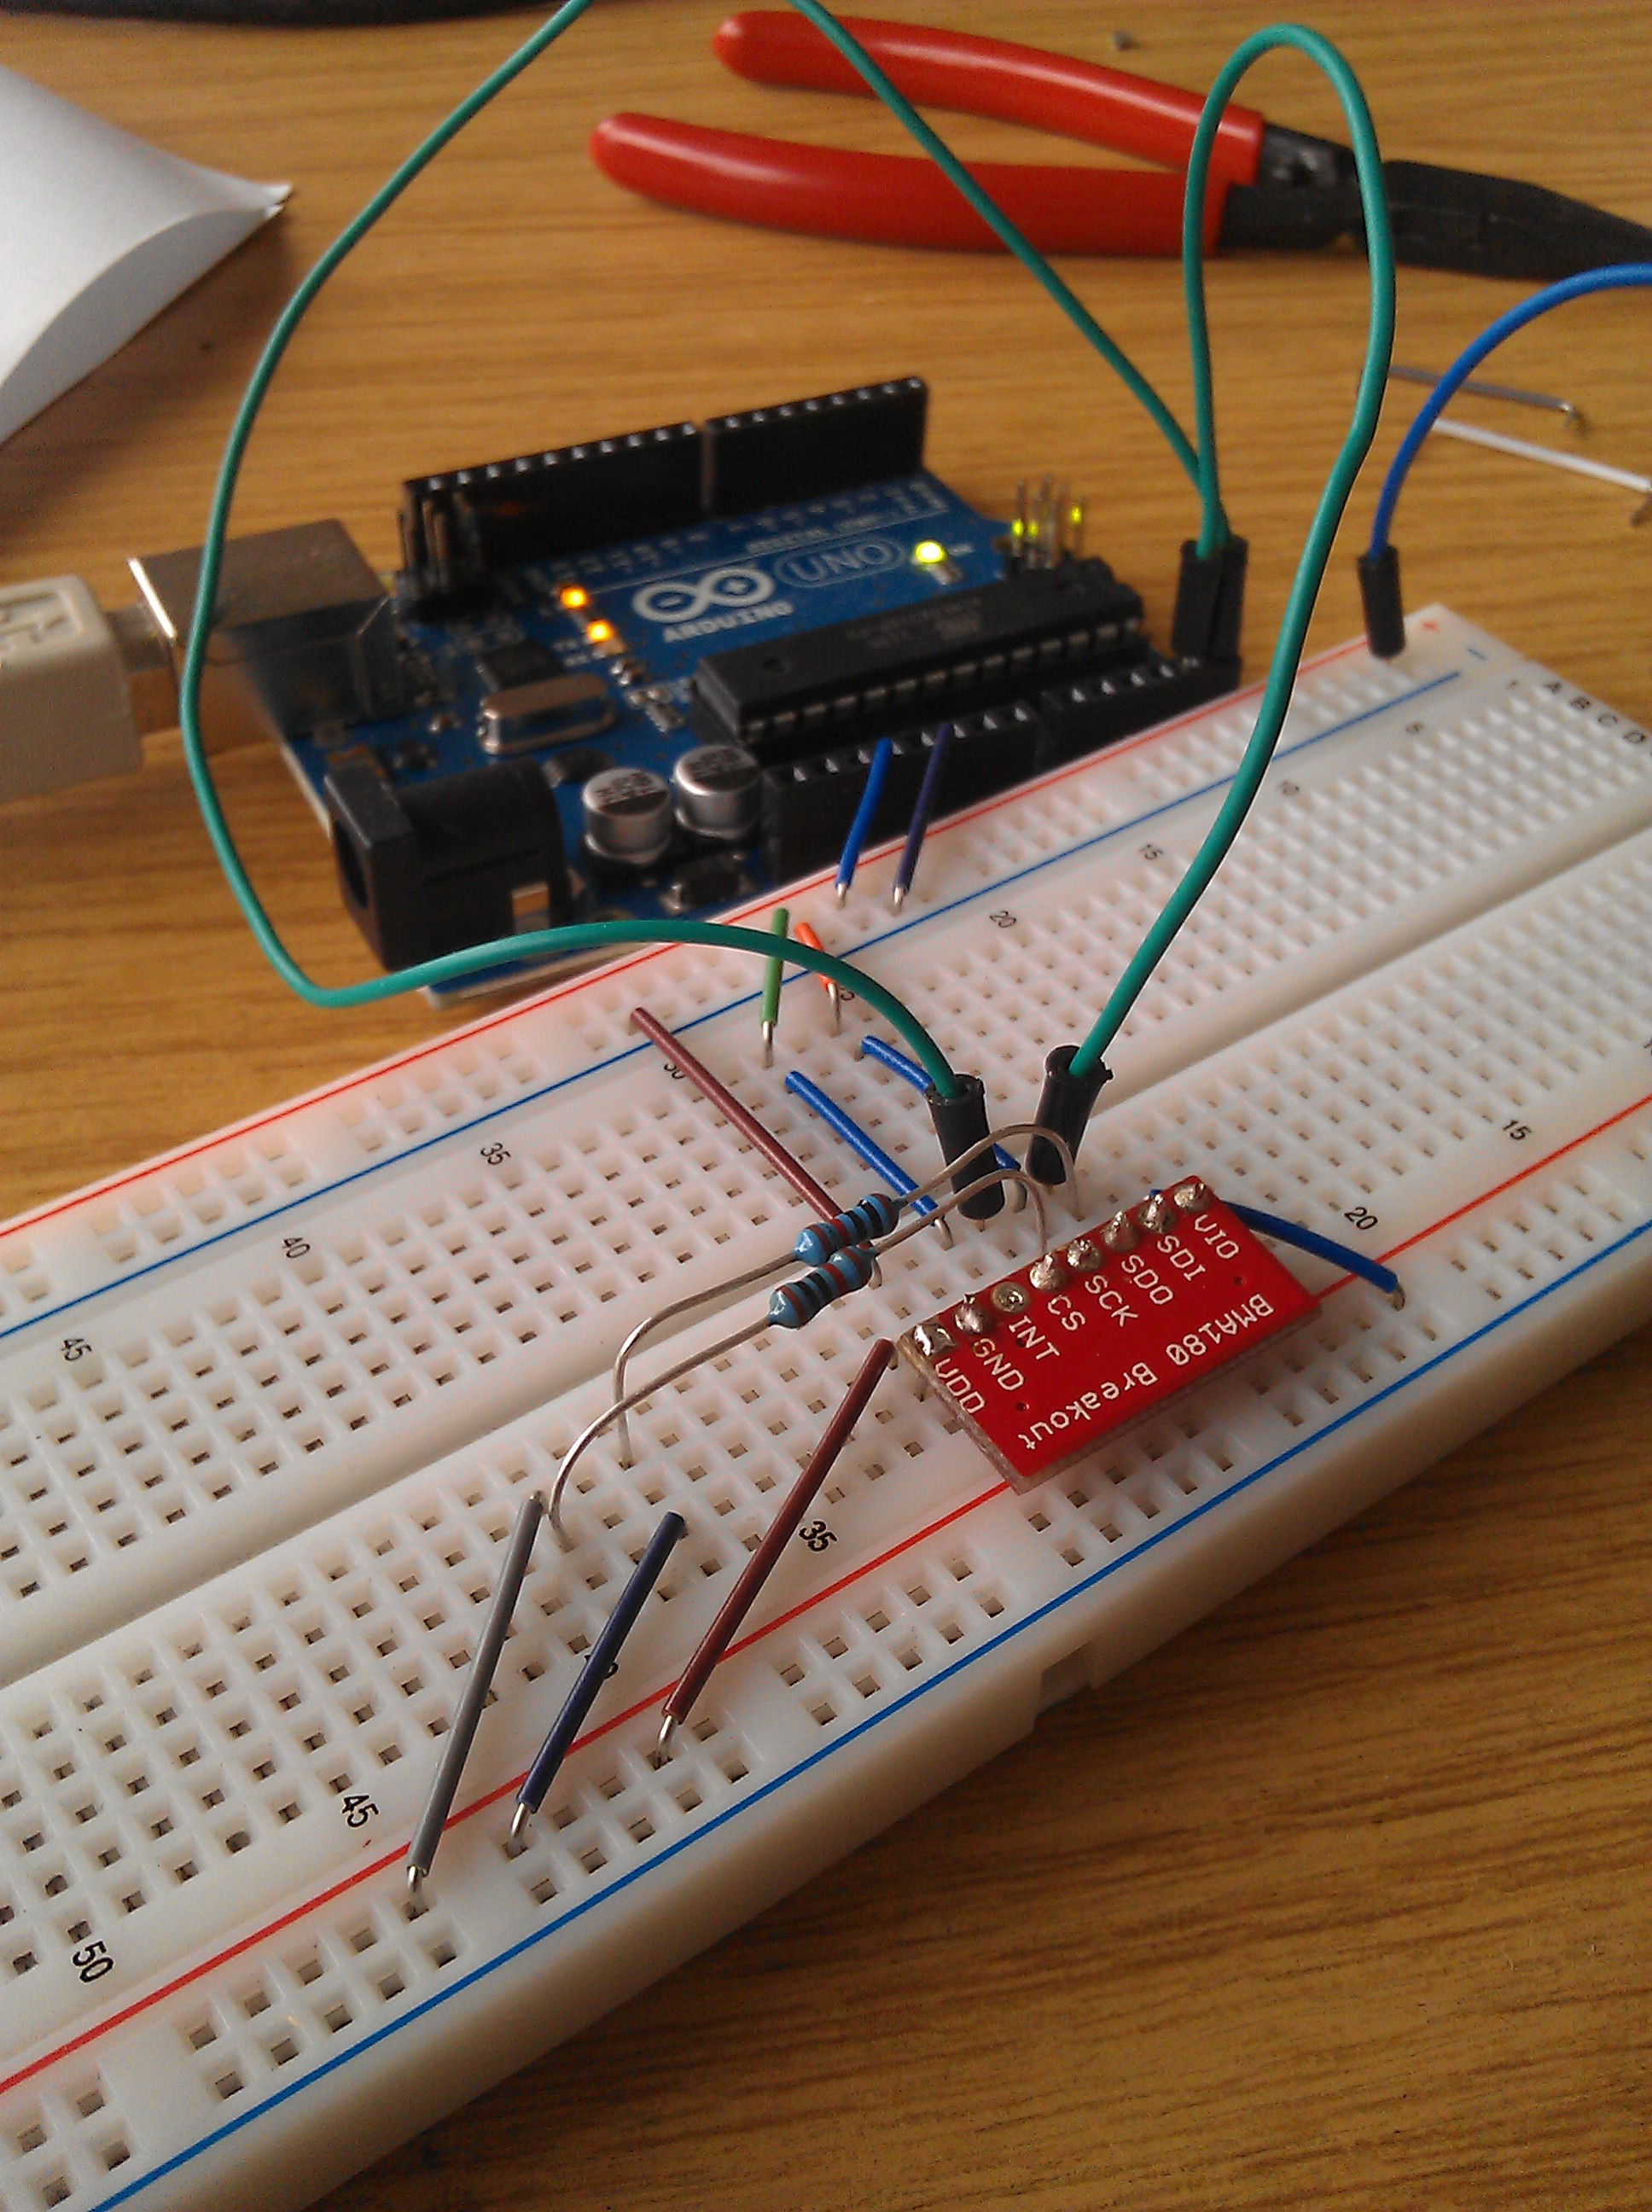
\includegraphics[scale=.111]{hardwareimages/breadboard.jpg}
	\caption{Testaufbau auf dem Breadboard}
	\label{breadboard}
\end{minipage}
\hfill
\begin{minipage}[H]{8cm}
	\centering
	\includegraphics[scale=.111]{hardwareimages/testaufbau.png}
	\caption{Testplatine am Radar}
	\label{testaufbau}
\end{minipage}
\end{figure}



\begin{table}[htb]
\begin{tabular}{@{}ll@{}}
      
      \cmidrule(r){1-2}\morecmidrules\cmidrule(r){1-2}
       SPI mode & I2C mode\\
      \midrule
 SDI input & SDA birectional (!) \\ 
 SDO output & ADDR adress bit, input \\
 SCLK input & SCL input \\
 CSB chip select, input & I2C mode select, input \\
   \addlinespace
   \bottomrule
 \end{tabular}
\caption{BMA180 Pinbelegung für SPI und I2C Modes \citep{Sensortec:2009rt}}
\label{i2cmode}
\end{table}


\begin{figure}[h]
\centering
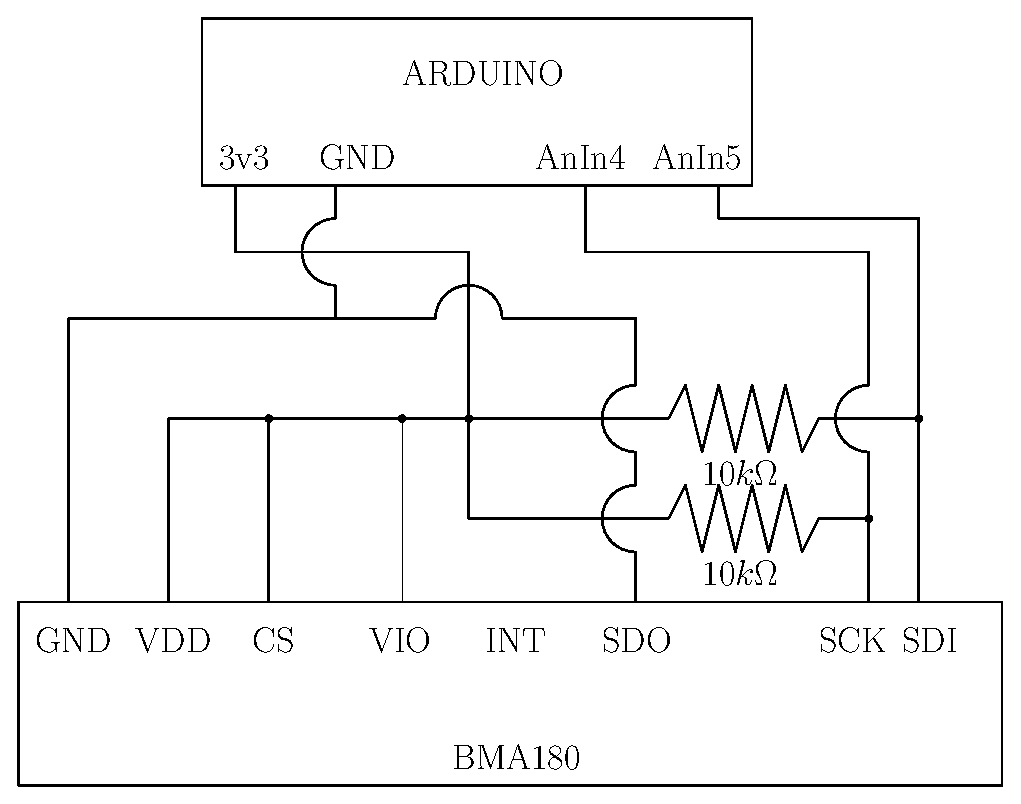
\includegraphics[scale=.8]{schematics.eps}
\caption{Schaltplan Testaufbau. Die Interrupts sind nicht verbunden, VCC und CS sind auf 3.3V geschaltet, GND und SDO auf die Masse des Arduinos gezogen, die I$^2$C Datenleitungen SCK und SDI sind mit den Arduinopins A4 und A5 verbunden, wobei zusätzlich 10k$\Omega$ Pull-Up-Widerstände eingebaut sind.}
\label{schematics}
\end{figure}


\newpage
\subsubsection{Fester Aufbau}

Um das System wirklich praktisch nutzen zu können muss er natürlich fest aufgebaut werden und mit einem Gehäuse versehen werden, das es erlaubt, ihn fest an einem Testobjekt anzubringen und ihn gleichzeitig vor Schäden durch mechanische oder witterungsbedingte Einflüsse schützt.

Um die eigentliche Sensoreinheit möglichst kompakt zu halten, habe ich mich entschieden, den Beschleunigungssensor vom Arduino zu trennen und auf eine kleine Lochrasterplatine zu löten. Diese wird in einen festen Block aus Polyurethanharz \citep{Components:2010fk} eingegossen, womit sie gleichzeitig gut geschützt und leicht anzubringen ist.

\begin{figure}[htb]
\centering
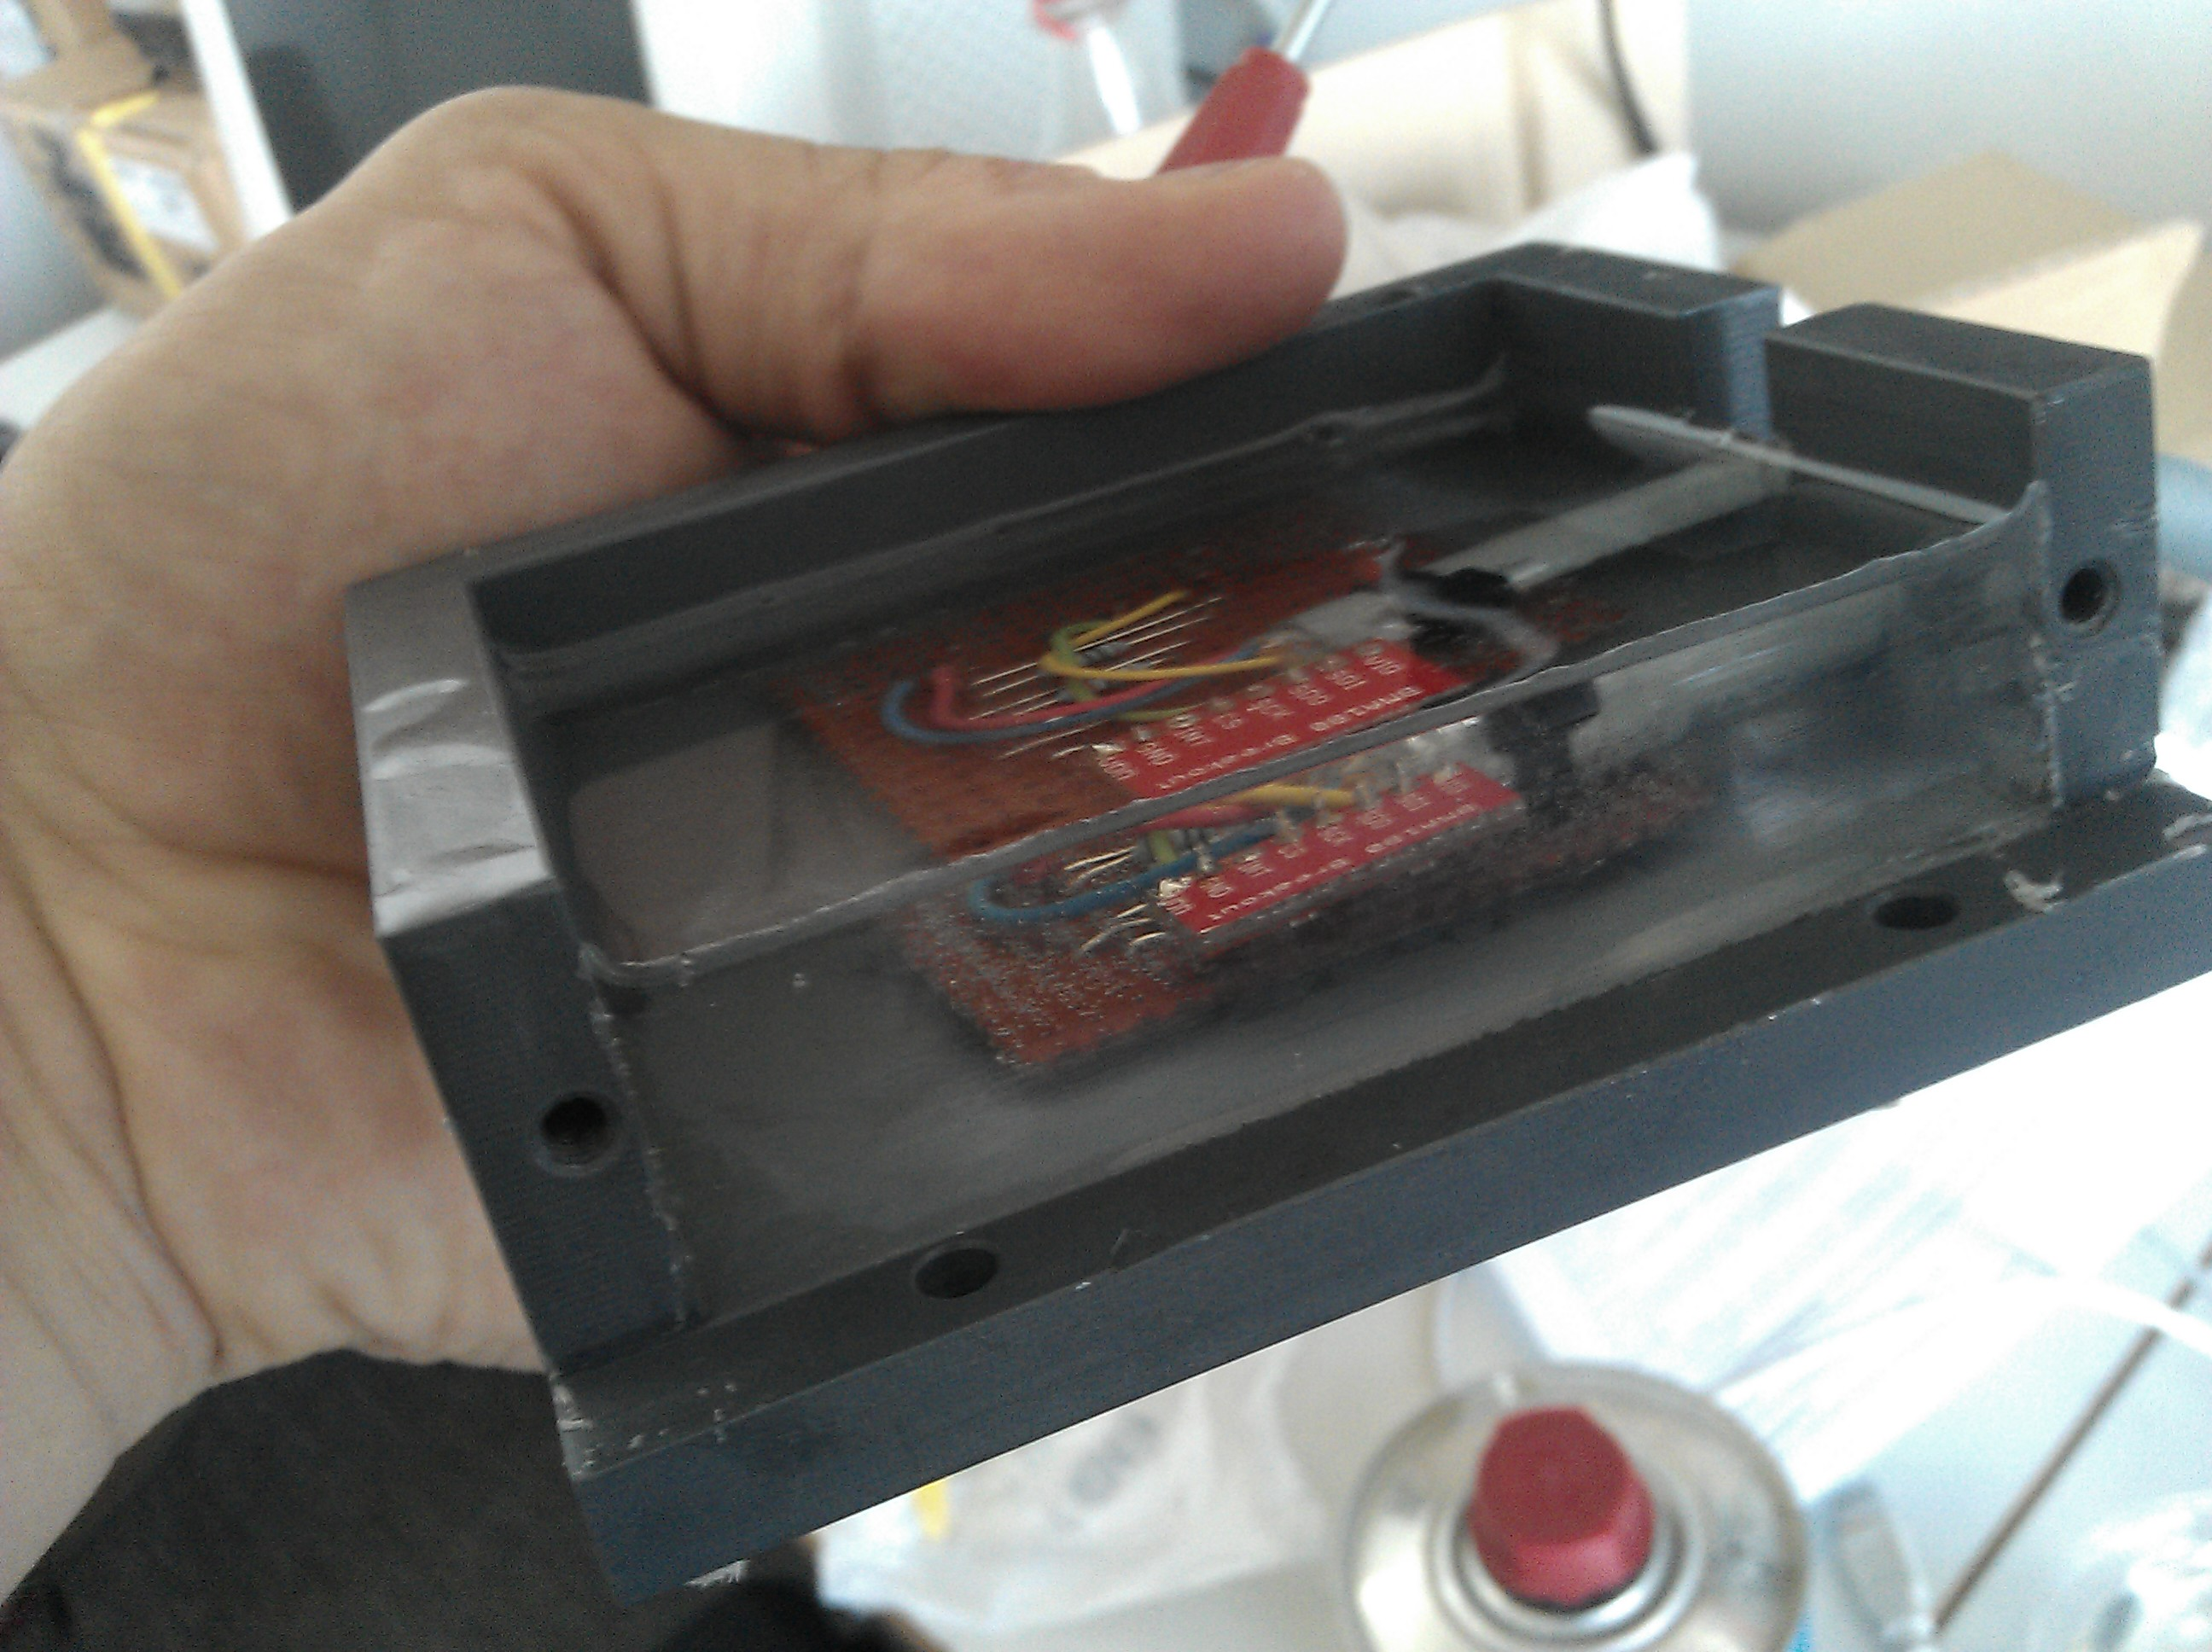
\includegraphics[scale=.15]{hardwareimages/harz.jpg}
\caption{BMA180 in Polyurethanharz eingegossen, die Kunststoffbox wurde von der technischen Werkstatt des Geomatikums gefertigt.}
\label{harz}
\end{figure}



\begin{figure}[htb]
\begin{minipage}[H]{8cm}
	\centering
	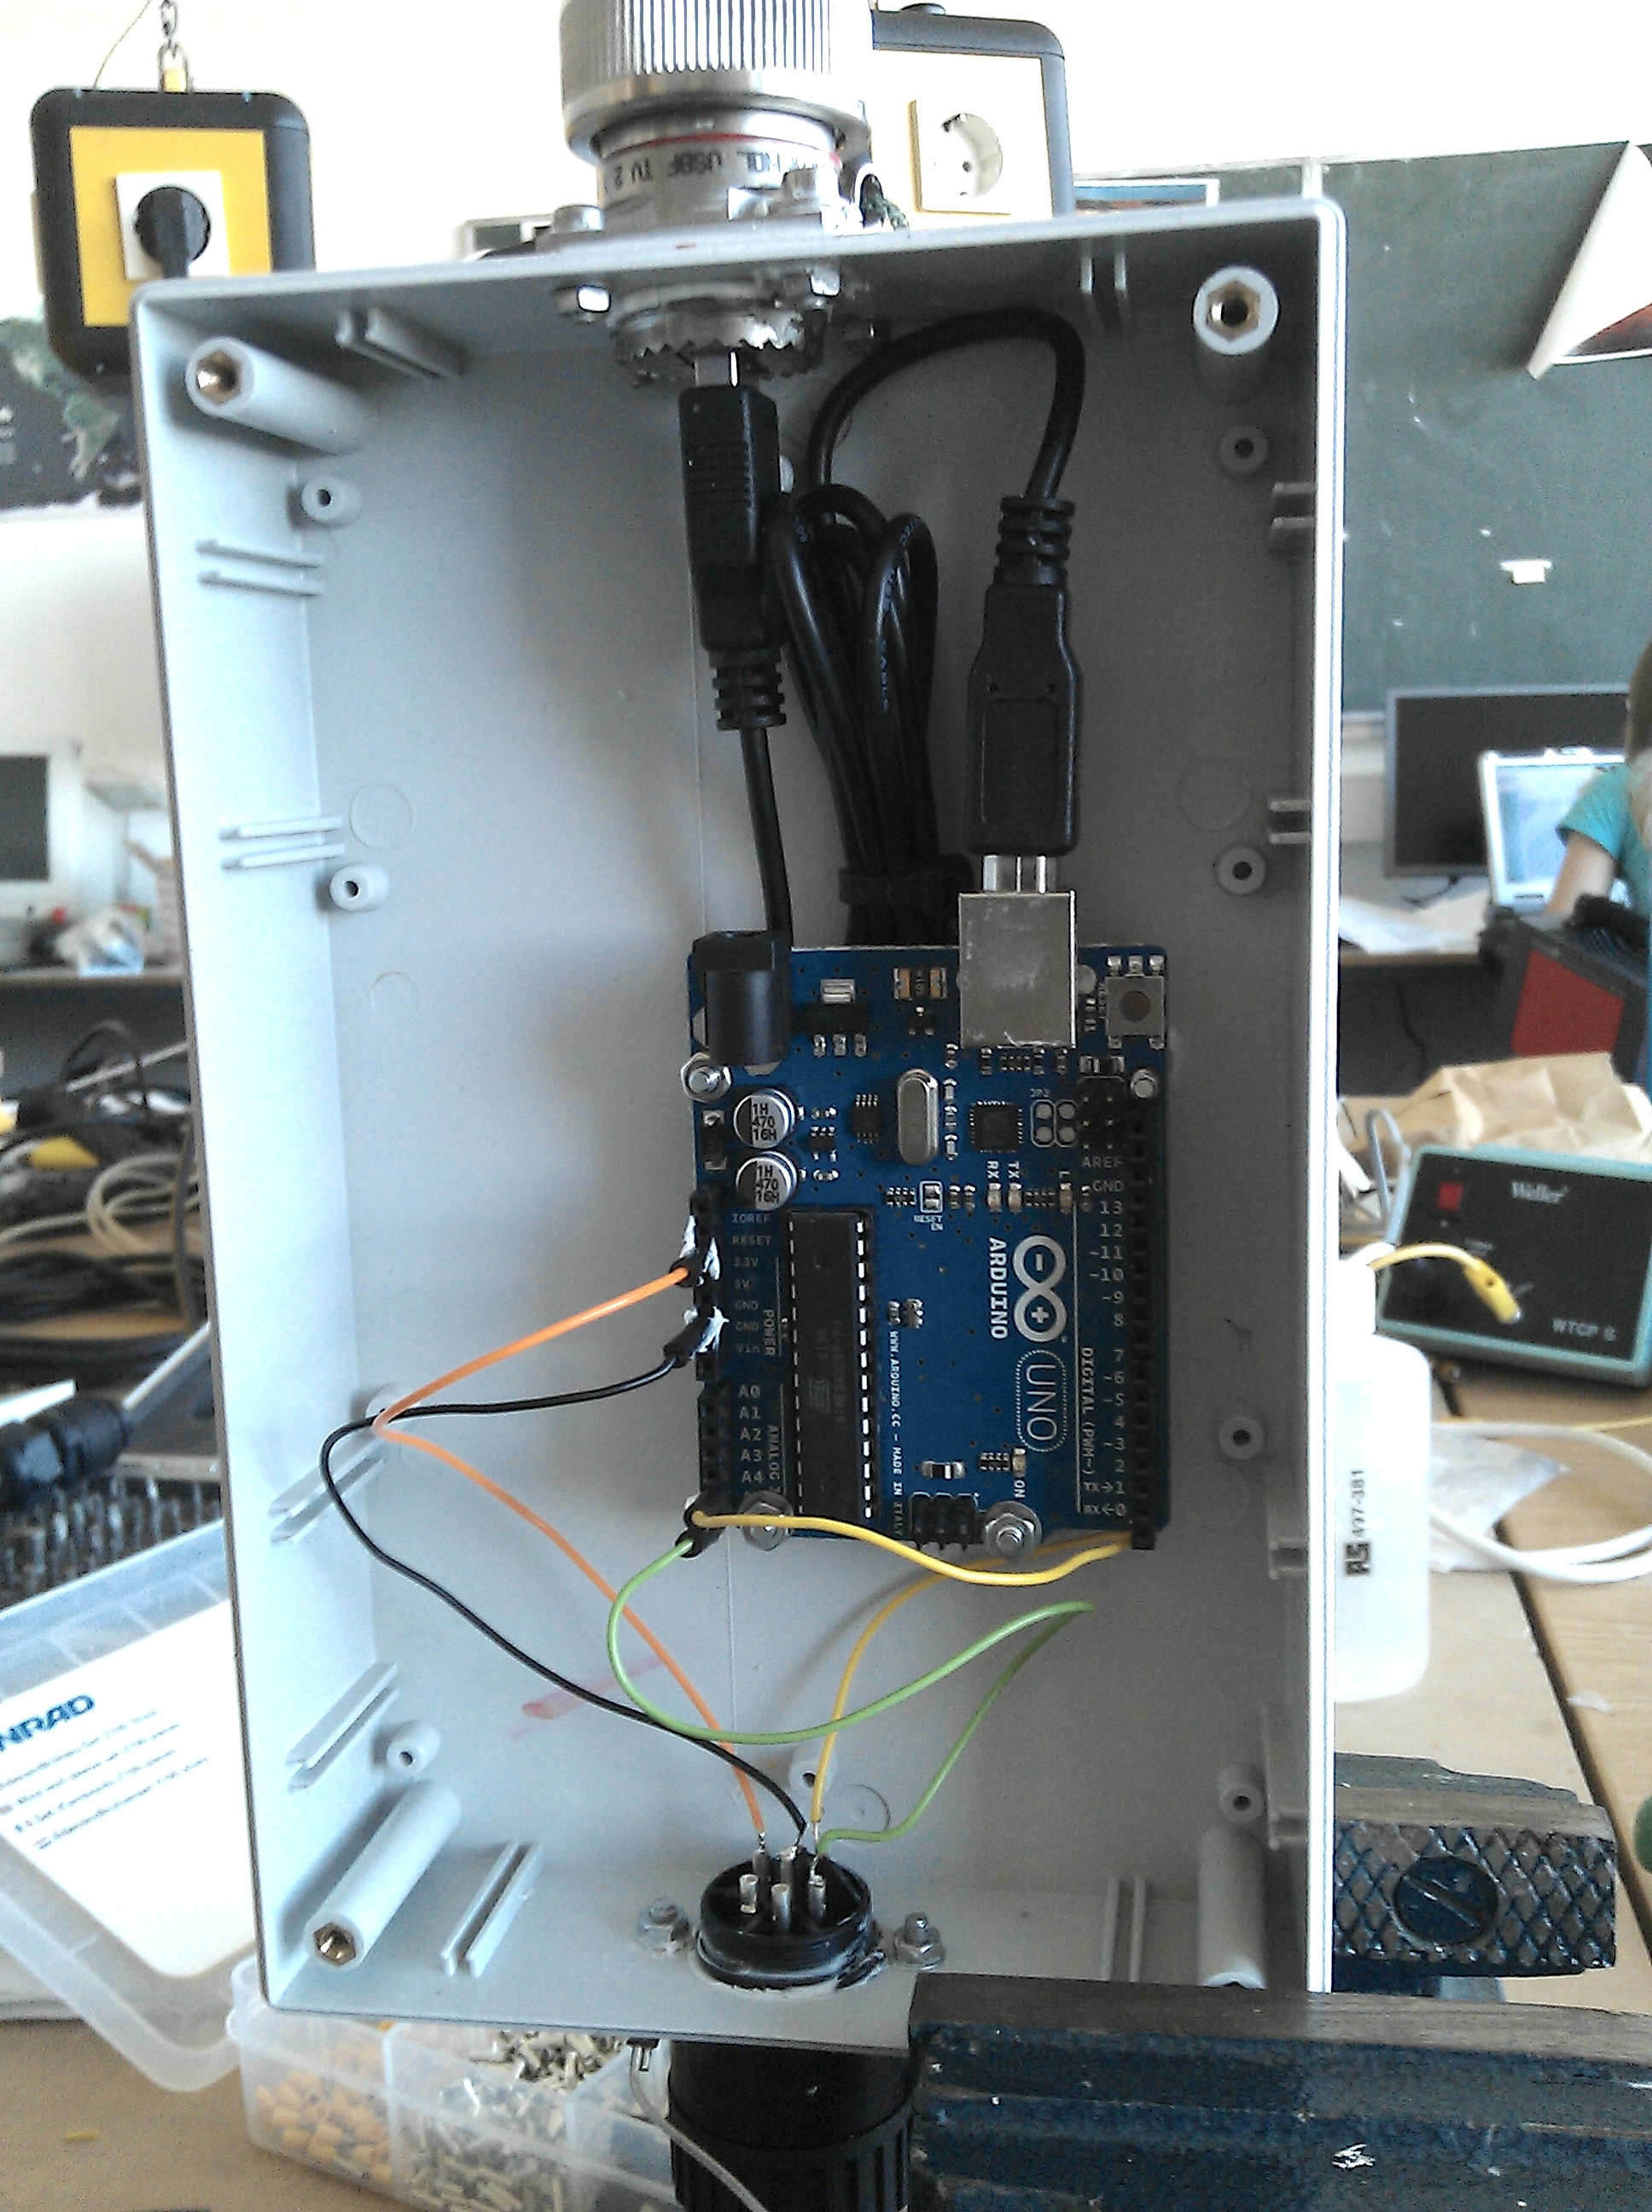
\includegraphics[scale=.111]{hardwareimages/arduinobox.jpg}
	\caption{Arduinobox}
	\label{arduinobox}
\end{minipage}
\hfill
\begin{minipage}[H]{8cm}
	\centering
	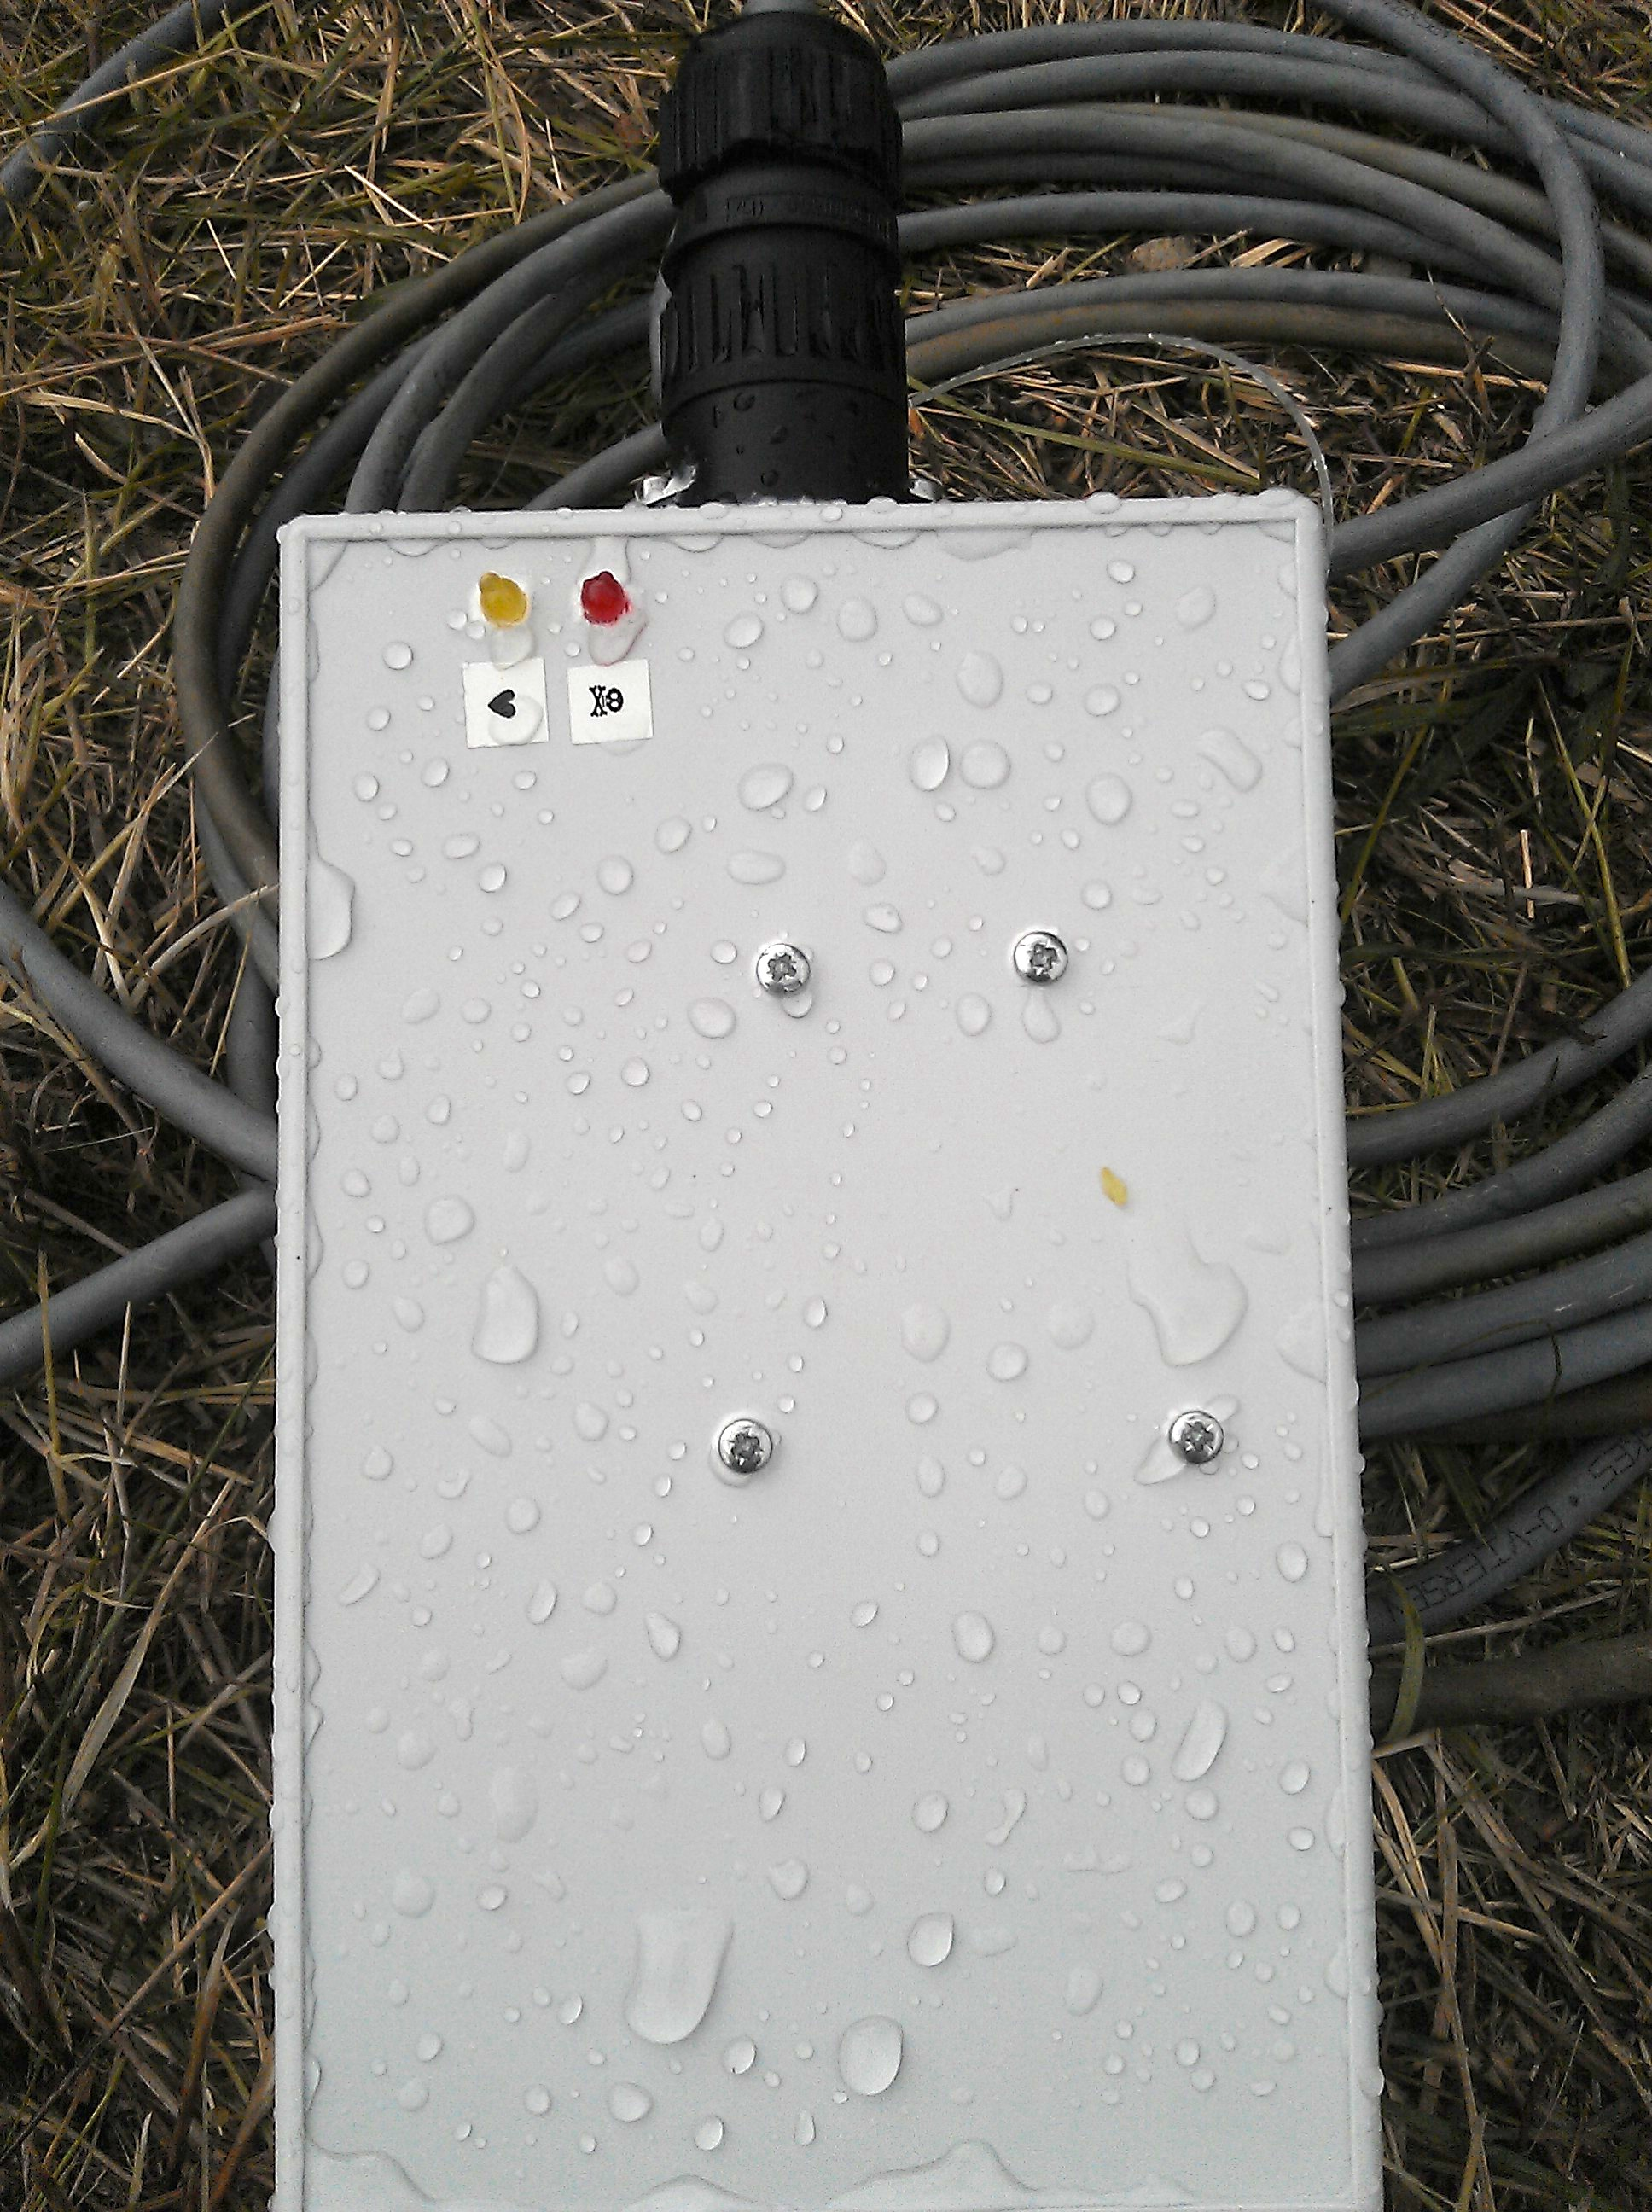
\includegraphics[scale=.111]{hardwareimages/arduinoboxregen.jpg}
	\caption{Arduinobox im Regen}
	\label{arduinoboxregen}
\end{minipage}
\end{figure}


\subsection{Software} 






\clearpage
\newpage
\appendix
\bibliographystyle{plainnat}
\bibliography{bachelor}









\end{document}
